% !TeX root = ../main.tex
% Add the above to each chapter to make compiling the PDF easier in some editors.

\chapter{Electrical Flows}

A classical graph problem is the flow of electrical currents through a network of resistors. Such a network $G = (\sV, \sE, \vx, \vr)$ can be described by a set of vertices $\sV$, set of wires (or edges) $\sE$, voltages $\vx \in \R^{|\sV|}$ at the vertices, and resistances $\vr \in \R_{>0}^{|\sE|}$ of wires. We are interested in finding the electrical flow $\vf \in \R^{|\sE|}$ through the network, assigning to each wire the current that is transported per unit time.

By \emph{Ohm's law}\index{Ohm's law}, we have that for any wire $e \in \sE$, \begin{align}
    \vf(e) = \frac{\vx(e)}{\vr(e)}, \quad \vx(e) = \vf(e) \cdot \vr(e),
\end{align} where $\vx(\{u,v\}) \defeq \vx(u) - \vx(v)$ is the voltage difference of vertices $u$ and $v$. The \emph{net flow}\index{net flow} of current at a vertex $u \in \sV$ is given as, \begin{align}
    \sum_{v \sim u} \vf(v, u).\margintag{We use $v \sim u$ to denote all $v$ that are adjacent to $u$.}
\end{align} We say that a flow routes \emph{demand}\index{demand} $\vd \in \R^{|\sV|}$ if the net flow at every vertex is $\vd(v)$. The fact that at vertices with zero demand, the flow is conserved\footnote{As much current is flowing into the vertex as is flowing out of it.} is also known as \emph{Kirchhoff's current law}\index{Kirchhoff's current law}.

\begin{marginfigure}
    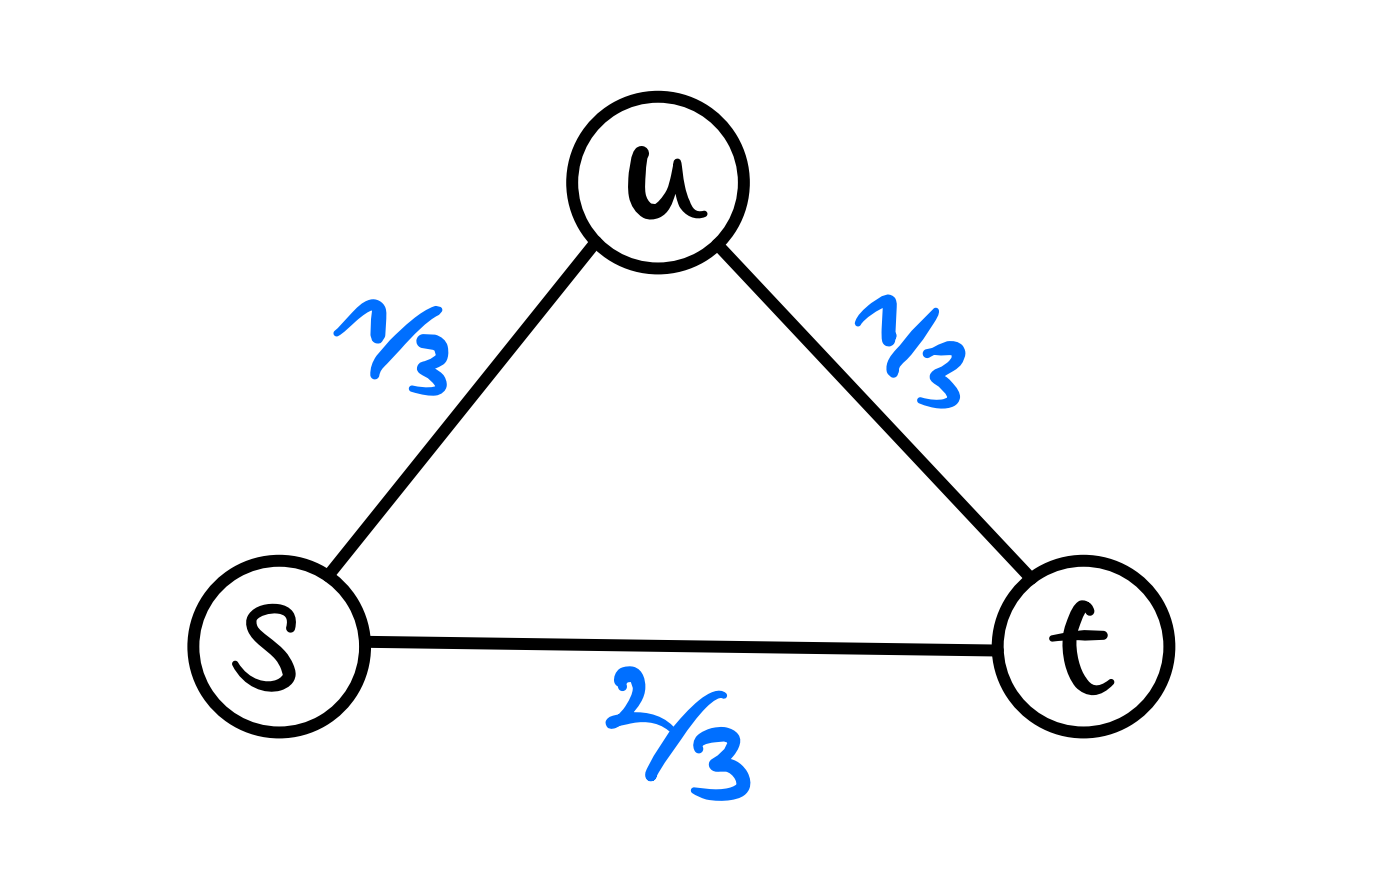
\includegraphics[width=\textwidth]{notes/figures/electrical_flows.png}
    \caption{Example of an electrical flow (shown in blue) with voltages \begin{align*}
        \vx(s) = 0,\quad \vx(u) = 1,\quad \vx(t) = 2
    \end{align*} and unit resistances, routing demands \begin{align*}
        \vd(s) = -1,\quad \vd(u) = 0,\quad \vd(t) = 1.
    \end{align*}}
\end{marginfigure}

To keep track of the direction of flow on each edge, we assign an arbitrary direction to each edge (we ``orient'' $G$) and only consider non-negative flows, $\vf \in \R_{\geq 0}^{|\sE|}$. Clearly, for any previously feasible flow, we can assign directions in such a way that the flow remains feasible.

\subsection{The Laplacian Matrix}

\begin{defn}[Adjacency matrix]\index{adjacency matrix}
The \emph{adjacency matrix} of a graph $G$, $\Tilde{\mA} \in \R^{|\sV|\times|\sV|}$, is defined as,\footnote{By $\mA$ we will later denote the weighted adjacency matrix.} \begin{align}
    \Tilde{\mA}(u, v) \defeq \begin{cases}
        1 & \text{if $u \sim v$} \\
        0 & \text{otherwise}.
    \end{cases}
\end{align}
\end{defn}
\begin{defn}[Incidence matrix]\index{incidence matrix}
The \emph{incidence matrix} of an oriented graph $G$, $\mB \in \R^{|\sV|\times|\sE|}$, is defined as, \begin{align}
    \mB(v, e) \defeq \begin{cases}
        1 & \text{if $e = (u,v)$ for some $u \in \sV$} \\
        -1 & \text{if $e = (v,u)$ for some $u \in \sV$} \\
        0 & \text{otherwise}.
    \end{cases}
\end{align}
\end{defn} Each column of $\mB$ only has two non-zero entries and sums to one.
\begin{marginfigure}
    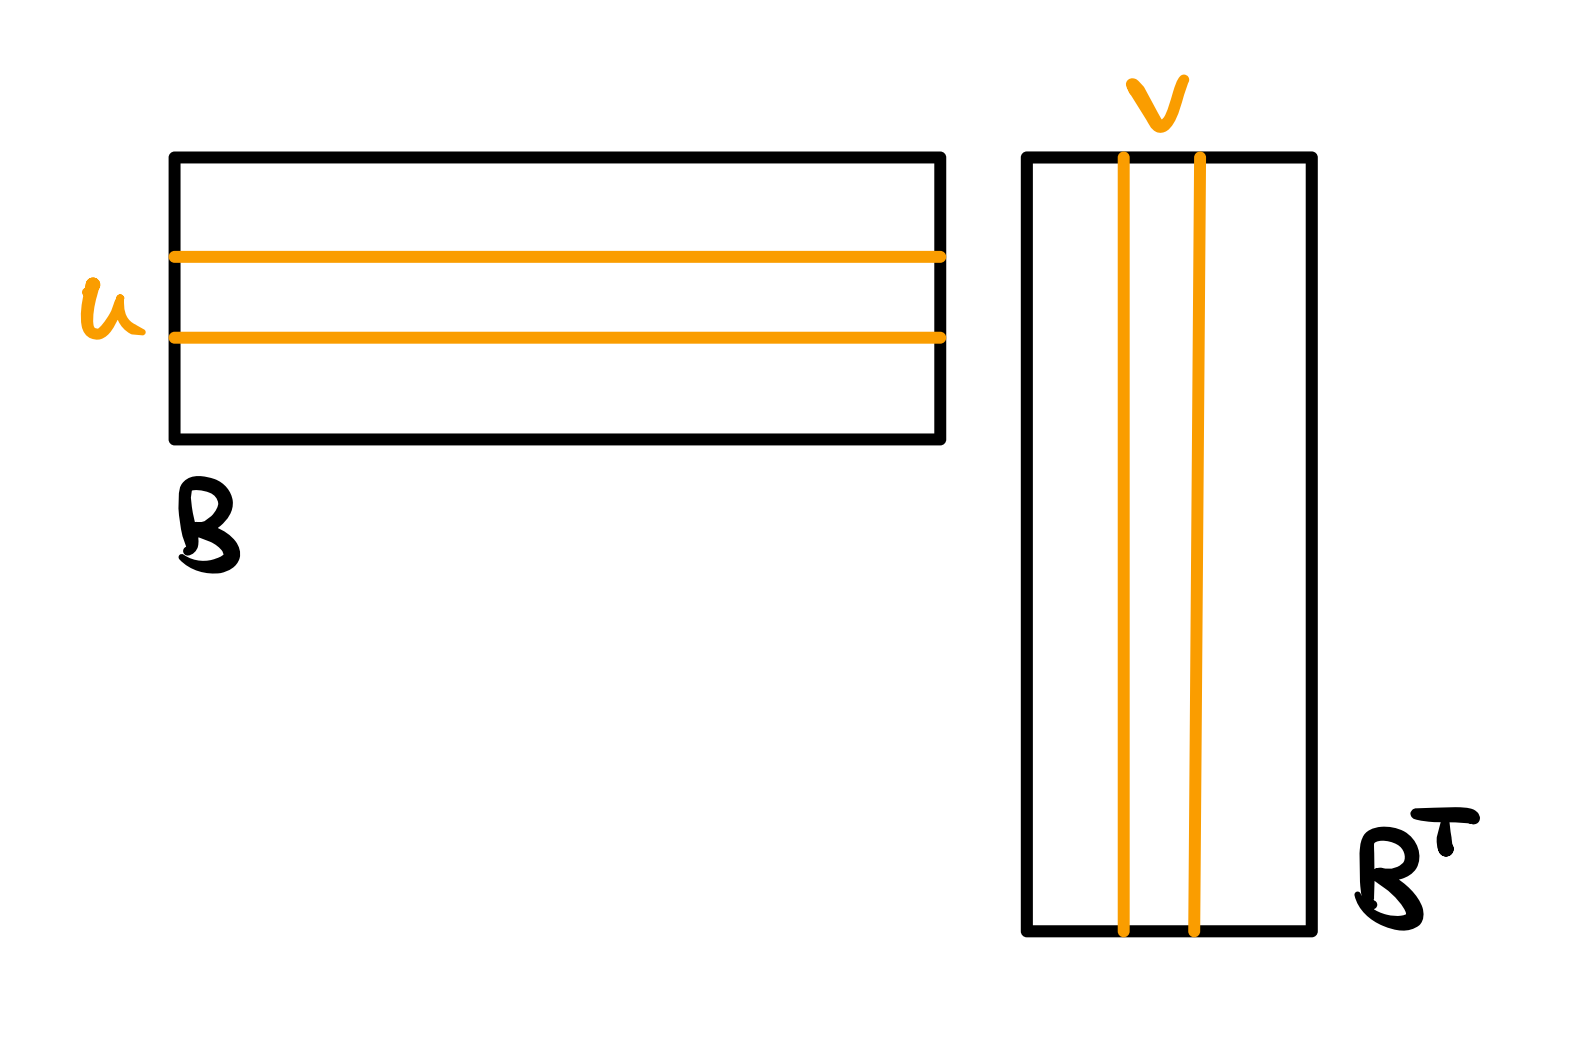
\includegraphics[width=\textwidth]{notes/figures/incidence_matrix.png}
    \caption{Illustration of the matrix product $\mB\trans{\mB}$.}
\end{marginfigure}
\begin{lem}\label{lem:incidence_matrix_product}
$\mB \trans{\mB} = \diag\{\deg(v)\}_{v \in \sV} - \Tilde{\mA}$.
\end{lem}
\begin{proof} The dot product of the rows, corresponding to the same vertex $v$, produces exactly $\deg(v)$. All other dot products between rows corresponding to vertices $u$ and $v$ are $-1$ iff $u \sim v$ and $0$ otherwise.
\end{proof}
We can now also write the net flow constraint\index{net flow constraint}, \begin{align}
    \mB\vf = \vd.
\end{align} We define $\mR \defeq \diag\{\vr(e)\}_{e \in \sE}$ and then have that Ohm's law\index{Ohm's law} can be expressed as, \begin{align}
    \trans{\mB}\vx = \mR\vf, \quad\text{or equivalently,}\quad \mR^{-1}\trans{\mB}\vx = \vf.
\end{align} If the net flow constraint is satisfied, this yields, \begin{align}
    \underbrace{\mB\mR^{-1}\trans{\mB}}_{\text{Laplacian}}\vx = \mB\vf = \vd.
\end{align}
\begin{defn}[Laplacian matrix]
The \emph{Laplacian matrix} of an oriented graph $G$, is defined as, \begin{align}
    \mL \defeq \mB\mR^{-1}\trans{\mB} = \mB\mW\trans{\mB} \in \R^{|\sV|\times|\sV|},
\end{align} where $\mW \defeq \mR^{-1}$ is a diagonal matrix of weights\index{weight (of an edge)} $\vw(e) \defeq \frac{1}{\vr(e)}$.
\end{defn}\noindent Intuitively, the weight of an edge can be understood as how ``connected'' the two vertices at its endpoints are. In contrast, the resistance of an edge is smaller when endpoints are well-connected.

We will now learn a little more about Laplacian matrices.
\begin{defn}[Weighted adjacency matrix]\index{weighted adjacency matrix}
The \emph{weighted adjacency matrix} of a graph $G$, $\mA \in \R^{|\sV|\times|\sV|}$, is defined as, \begin{align}
    \mA(u, v) \defeq \begin{cases}
        w(\{u,v\}) & \text{if $u \sim v$} \\
        0 & \text{otherwise}.
    \end{cases}
\end{align}
\end{defn}
\begin{lem}
$\mA$ is symmetric, that is, $\mA = \trans{\mA}$.
\end{lem}
\begin{proof}
This follows immediately from the fact that $G$ is undirected.
\end{proof}
\begin{defn}[Weighted degree]\index{weighted degree}
The \emph{weighted degree} of a vertex $v \in \sV$ is given as, \begin{align}
    \vw(v) \defeq \sum_{\{u,v\} \in \sE} \vw(\{u,v\}).
\end{align} We write $\mD \defeq \diag\{\vw(v)\}_{v \in \sV}$.
\end{defn}

\begin{lem}
$\mL = \mD - \mA$.
\end{lem}
\begin{proof}
The proof is identical to the proof of \cref{lem:incidence_matrix_product}, only that every entry is now weighted, due to the additional factor $\mW$.
\end{proof}

\begin{lem}
For any $\vx \in \R^{|\sV|}$, we have, \begin{align}
    \trans{\vx}\mL\vx = \sum_{\{u,v\}\in\sE} \vw(\{u, v\})[\vx(u) - \vx(v)]^2 \geq 0.
\end{align}
\end{lem}
\begin{proof}
We have, \begin{align*}
    \trans{\vx}\mL\vx &= \trans{\vx}\mD\vx - \trans{\vx}\mA\vx. \\
    \trans{\vx}\mD\vx &= \sum_{v \in \sV} \vw(v) \vx(v)^2 = \sum_{\{u,v\}\in\sE} \vw(\{u,v\})[\vx(u)^2 + \vx(v)^2]. \\
    \trans{\vx}\mA\vx &= \sum_{v \in \sV} \vx(v) (\mA\vx)(v) \\
    &= \sum_{v \in \sV} \vx(v) \sum_{u \in \sV} \mA(v,u) \vx(u) \\
    &= \sum_{v,u \in \sV} \vw(\{u,v\})\vx(u)\vx(v) \\
    &= 2 \sum_{\{u,v\}\in\sE} \vw(\{u,v\})\vx(u)\vx(v).
\end{align*} Combining the above equalities, we obtain, \begin{align*}
    \trans{\vx}\mL\vx &= \sum_{\{u,v\}\in\sE} \vw(\{u,v\})[\vx(u)^2 + \vx(v)^2] - 2 \sum_{\{u,v\}\in\sE} \vw(\{u,v\})\vx(u)\vx(v) \\
    &= \sum_{\{u,v\}\in\sE} \vw(\{u,v\})[\vx(u) - \vx(v)]^2. \qedhere
\end{align*}
\end{proof}
\begin{cor}
$\mL$ is positive semi-definite.
\end{cor}

\subsection{Framed as an Optimization Problem}

\subsection{Energy \& Duality}

\subsection{Outlook: More Graph Optimization Problems}